\documentclass[30pt, a1paper, portrait, margin=0mm, innermargin=15mm,blockverticalspace=15mm, colspace=15mm, subcolspace=8mm]{tikzposter} 
	\usepackage{graphicx}
	\usepackage{subcaption}
	\usepackage{caption}
	\usepackage{natbib}
	\usepackage{hyperref}

    \title{Attacking Microcontrollers} 
    \institute{Schoold of Electronics and Computer Science, University of Southampton}
    \author{Author: Dionisio Perez-Mavrogenis (dpm3g10)\\
			Supervisor: Klaus-Peter Zauner (kpz)}
    \usetheme{Board} %Board is also cool

    
\definebackgroundstyle{die_image}{
\includegraphics[height=\paperheight, width=\paperwidth]{opt.jpg}
}
\usebackgroundstyle{Rays}    
    
\begin{document}

	\maketitle     
    \begin{columns} % See Section 4.4
        \column{0.5} % See Section 4.4
            \block{Microcontroller Introduction}{
                Microcontrollers can be found anywhere, from your cars stereo to missile launch panels and are usually cheap (around \pounds 2) and packed with information! They often come with crypto-engines (AES, DES and RSA are common) and hold all sorts of information like private crypto-keys for authentication or propietary algorithm implementations in the firmware or hardware, interesting all sorts of people into the contents of a microcontroller.
                
                \textbf{insert cool graphic here}
            }
            \block{Packaging and De-packaging}{
				Typically microcontrollers are too small and fragile to use as they are fabricated (with fabrication lengths shrank to micro-meters) and so they are packaged\citep{hwre}. Packacking material ranges depending on the microcontroller and its intended use,  but is usually hard epoxy resin \citep{sergei:thesis} \citep{hwre}. The packaging tries to protect the microcontroller from its external environment (humidity, radiation, temperature, crashes etc.) and also from prying eyes. Military-grade chips come with a lot of additional circuitry on the packaging whose responsibility is to detect tampering and respond in a suitable manner (even self destruction!) \citep{hwre}.\\
               De-packaging is not always requierd and the methods depend on the packaging used and protective mechanisms in place, but on epoxy-packaged chips one can etch the epoxy away by using HNO$_3$ or H$_2$SO$_4$ and then cleaning the chip in an ultrasonic bath \citep{sergei:thesis} \citep{hwre}. For other packaging types, e.g. metal, ceramic or plastic, one can use similar techniques and tools, e.g. drills or a blowtorch \citep{hwre}.
               		
	
		\begin{minipage}{0.5\linewidth}
			\begin{tikzfigure}[ATmega328 with epoxy resin packaging.]
				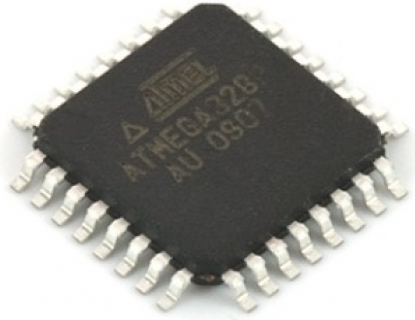
\includegraphics[width=0.7\textwidth]{atmega328.jpg}
			\end{tikzfigure}
		\end{minipage}% <--- the percent character will "comment out" the new line    
		\begin{minipage}{0.5\linewidth}
			\begin{tikzfigure}[The exposed die of an ATmega328.]
				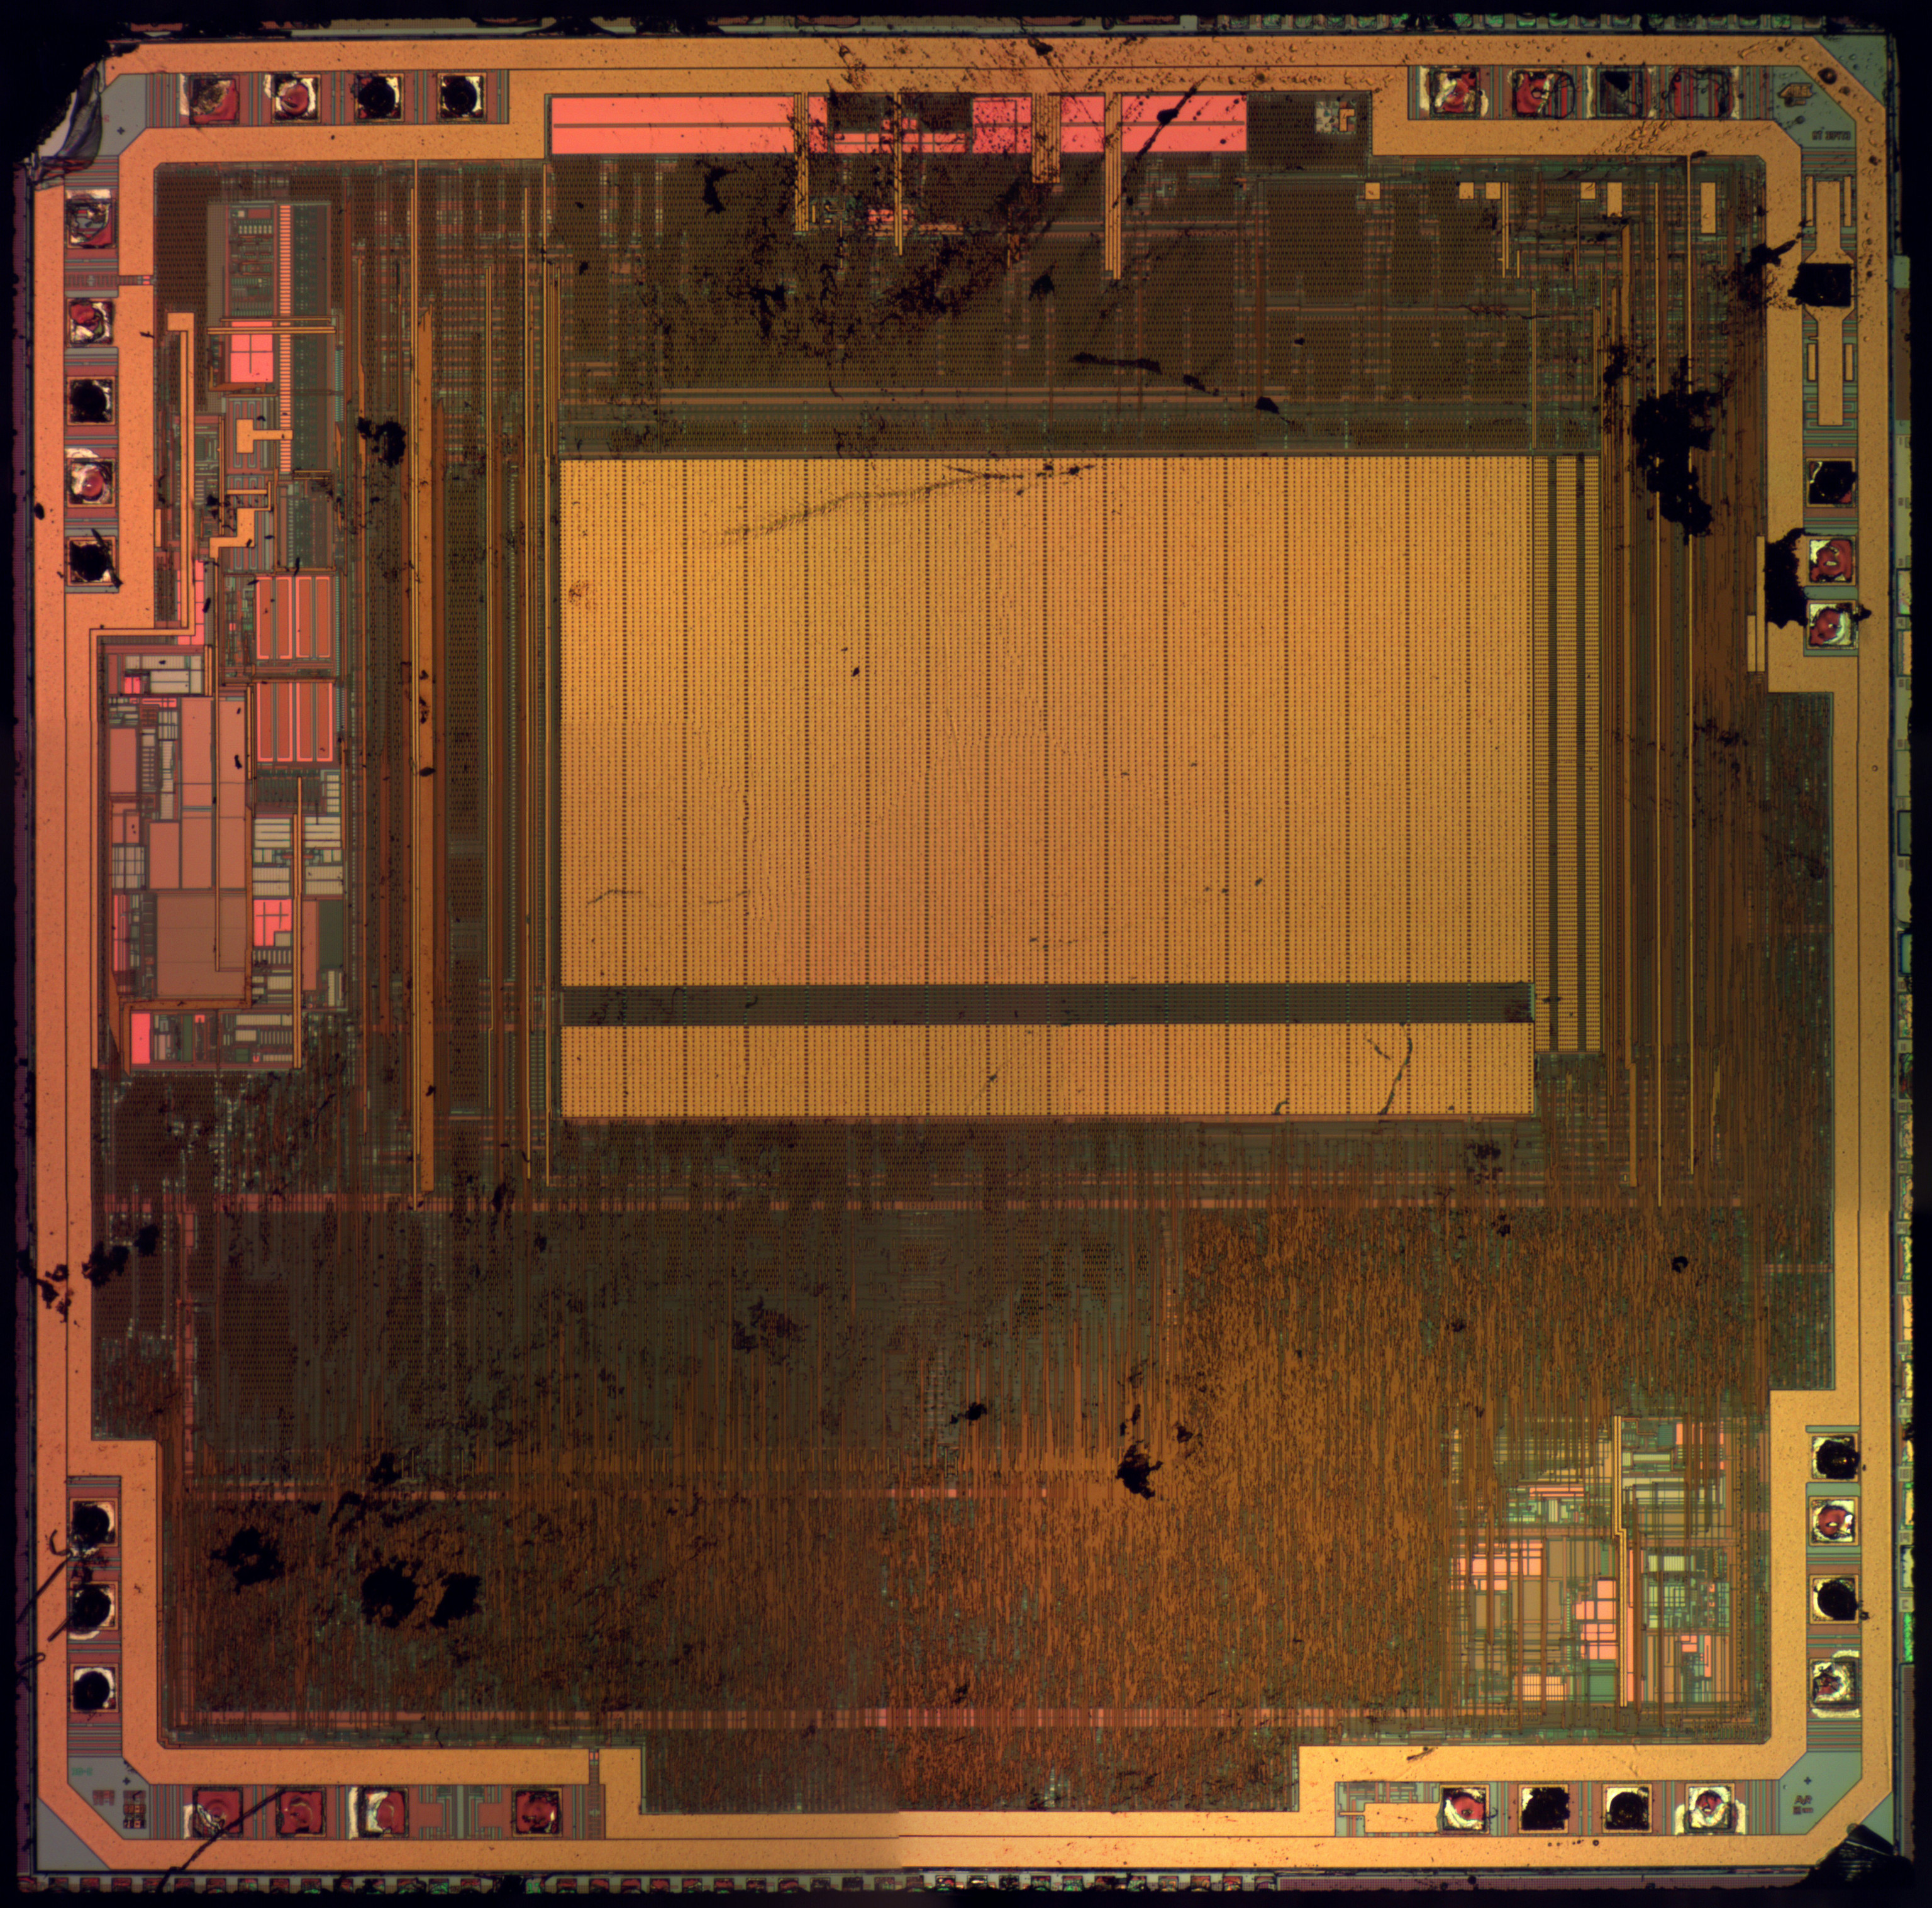
\includegraphics[width=0.7\textwidth]{atmega328_open.jpg}
			\end{tikzfigure}
		\end{minipage}
               
          }% end block
                 

            \note[rotate=15, width=15cm, targetoffsetx=5cm,targetoffsety=-5cm]{tampering detection means detecting abnormalities in voltage, clock frequency, radiation, tilting etc.}
                
        \column{0.5}
        	\block{Attack Types}{
				\textbf{Non-Invasive} attacks require no depackaging and are cheap to implement. Popular methods in this category are power analysis and fault injection, where faults may be injected by excessively heating the chip, underclocking or overclocking, using a lot more or a lot less voltage the the chip supports and more. Although these attacks are conceptually easy and do not require expensive hardware to perform, they are tricky to defend from. 
				\draw[ycomb,
color=gray,
line width=0.5cm]
plot coordinates{(1,1) (2,2) (3,3)};
				\textbf{Semi-invasive and Invasive} attacks require decapsulation and are a lot more technical, expensive (to perform and repliate) and time consuming with manufacturer-equivalent machinery used. 
        	}
            \block{Sample Attack}{
                provide atmega644 characteristics.
                set attack scenario, type, setup and exact details
            }
            \block{Evaluation}{
                Shit be broken, yo.
                \innerblock{qwgfwg}{qgwwg}
            }
        \note[rotate=15]{
			Very sexy, this is.        
        } % See Section 4.3
    \end{columns}
    
\bibliographystyle{plain}
    
    \block[roundedcorners=65]{}{{\footnotesize \bibliography{irp_report}}}
\end{document}